\section{Benchmark: block size versus write speed}
\label{sec:blocksize}
The Wupper GUI makes it possible for the users to configure the block size value. This appendix shows how much effect the block size have on the write speed. 

During a DMA write action (FPGA$\,\to\,$PC), a transfer request is transferred from the host to the FPGA, therefore a write descriptor is setup. This descriptor contains information such as memory addresses, direction and the size of the payload, i.e. the amount of data to be transfered. The descriptor is then handled by Wupper, and the data transfer to host initiated. The size of the payload is in this case also the block size. For example when users choose to have a block size of 1 KB, the request gets completed after 1 KB of data had been transferred to host. Subsequently a new header will be created and repeated until the throughput measurement is stopped by the user. 
A plot of the block size versus write speed is shown below in Figure~\ref{fig:blocksizeplot}. One can clearly observe from this plot that the block size have effect on the write speed. This is somehow expected as there is an overhead due to the request of those blocks, hence the more data get transfer per request, the better the PCIe bandwidth is exploited. The bigger the block size is, the faster the write speed gets. The throughput obviously saturates at a level close to the theoretical maximum speed defined by an 8 lane PCIe Gen3 link (64 Gbps).

\begin{figure}[h]
	
	\centering
	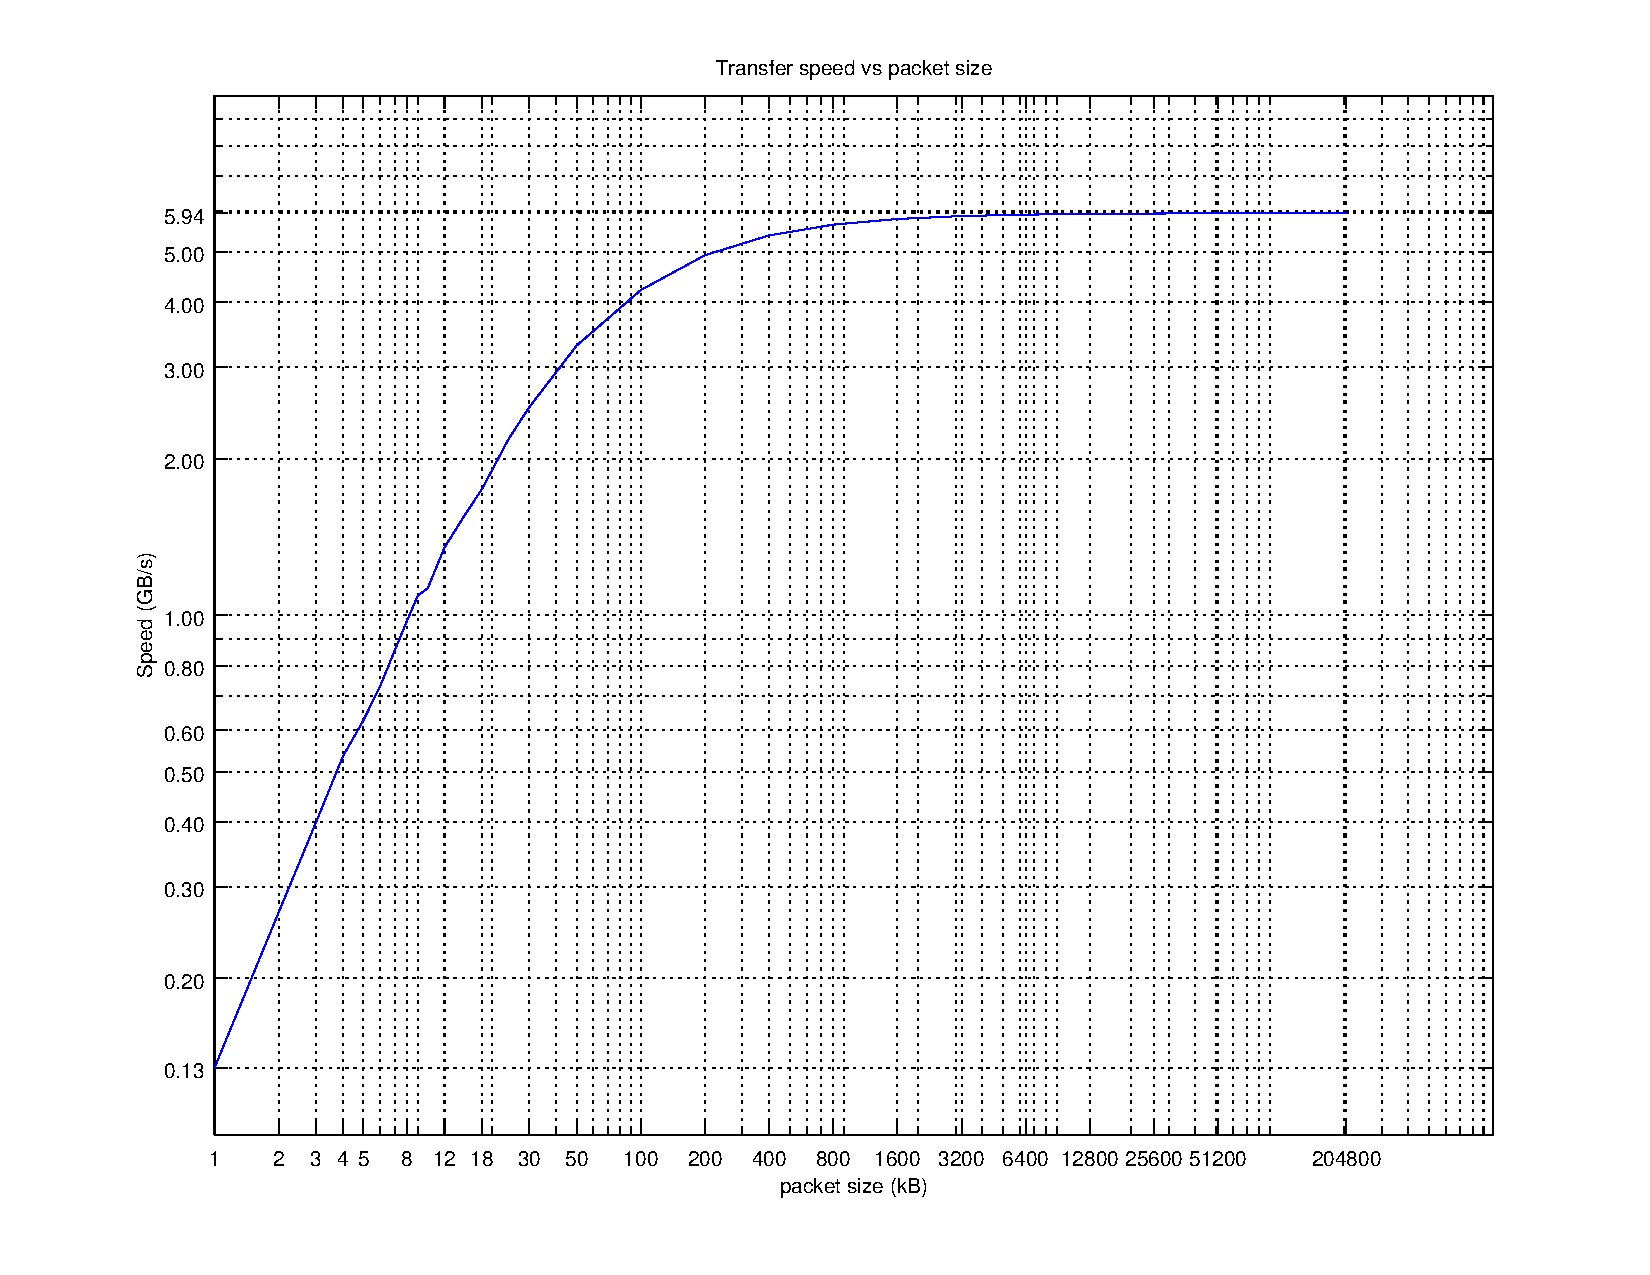
\includegraphics[width = 1 \textwidth]{figures/blocksize_plot.pdf}	
	\caption{Transfer speed vs packet size}
	\label{fig:blocksizeplot}
\end{figure}